\section{Durchführung}
\label{sec:DurchführungSchall} % bitte dort hinpacken wo du die Laufzeitmessung erklärst :))

\subsection{Durchbiegung eines einseitig und beidseitig eingespannten homogenen Stabes}
Um die Biegung der Stäbe zu messen wird folgende Apparatur verwendet.\\
\begin{figure}[H]
    \centering
    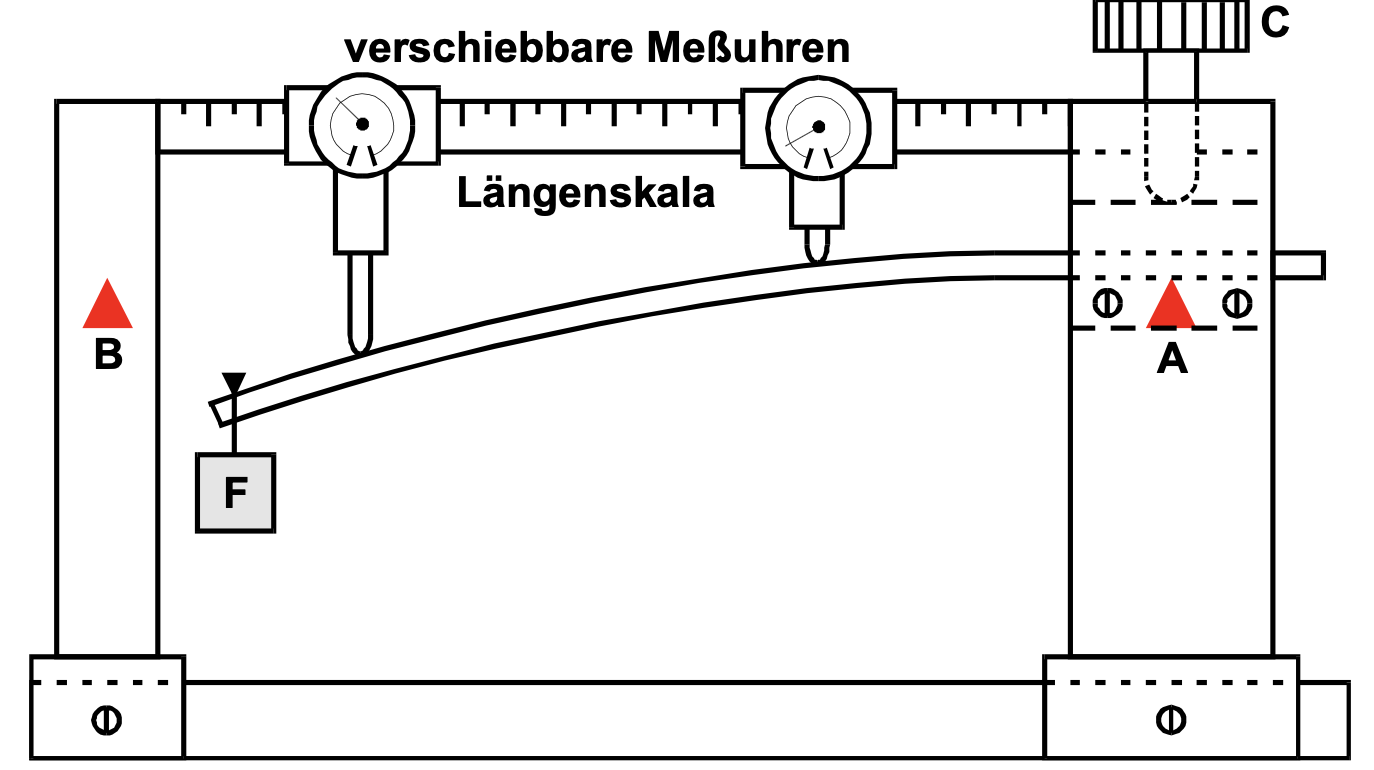
\includegraphics[width=0.8\textwidth]{BiegungA.png}
    \caption{Schematische Darstellung einer Apparatur zur Vermessung elastisch gebogener Stäbe\cite{v103_anleitung}}
    \label{fig:BiegungA}
\end{figure}
\subsubsection{Durchbiegung eines einseitig eingespannten homogenen Stabes}
Für die Durchbiegung eines einseitig eingespannten homogenen Stabes, wird der Stab einseitig (Abbildung \ref{fig:BiegungA} rechts) eingespannt. Anschließend wird das Gewicht am freien Stabende angebracht. Dabei wird die Last so gewählt, dass der Stab elastisch verformt wird und eine maximale Durchbiegung zwischen 3 und 7 \unit{\milli\meter} entsteht.\\
Die Auslenkung wird an verschiedenen Stellen entlang einer Längenskala mit einer verschiebbaren Messuhr über deren federnde Taststifte gemessen. Ein Teilstrich entspricht dabei einer Verschiebung von 10 \unit{\micro\meter}. 
Da weder der unbelastete Stab absolut gerade noch die Führung der Messuhren exakt parallel zur Stabachse ausgerichtet ist, nimmt man an jeder Messstelle zuerst den Ausgangswert ohne Gewicht und danach den Wert unter Last.\\
Die tatsächliche Durchbiegung ist also: $ D(x) = D_m (x) – D_0(x)$ \\
Dieses Vorgehen führen wir sowohl für einen Stab mit zylindrischem als auch für einen mit rechteckigem Querschnitt durch, um die Durchbiegung $D(x)$ in Abhängigkeit von x zu messen \cite{v103_anleitung}.\\
\subsubsection{Durchbiegung bei beidseitig eingespanntem homogenem Stab}
Für diesen Versuchsaufbau spannen wir einen Probestab beidseitig auf zwei Stützpunkten ein. Anschließend wird das Gewicht bei beidseitiger Lagerung in der Stabmitte angebracht. \\
Mithilfe zweier verschiebbarer Messuhren wird die Auslenkung an mehreren Positionen entlang einer Längenskala gemessen, wobei beide Messuhren stets denselben Abstand zueinander einhalten. \\
Auch hier wird an jeder Stelle zuerst der Nullwert $D_0 (x)$ ohne Last und dann der Wert $D_m (x)$ unter Last abmessen. Die tatsächliche Durchbiegung ergibt sich dann wieder durch die Differenz \cite{v103_anleitung}.\\
\subsection{Laufzeit von Schallimpulsen}
Wir bestimmen nun die Laufzeit von Schallimpulsen mit dem zuvor erläuterten Apparat. Dafür legen wir jeweils den Stab in die Vorrichtung (siehe Abbildung \ref{fig:SchallwellenA}) und setzten vor jedem Durchgang die Messanzeige zurück.\\
\subsection{Bestimmung der geometrischen Abmessungen und Massen}
Beide Stäbe werden mit einer Waage gewogen. Für den rechteckigen Stab bestimmen wir die Kantenlänge mithilfe einer Schiebelehre, beim runden Stab entsprechend der Durchmesser. Für die Längen wird ein Maßband verwendet.\\

